\documentclass[paper=a6,landscape,ngerman,twoside=true,fontsize=12pt]{scrartcl}
% % % Zeichenkodierung und Sprache % % %
\usepackage[utf8]{inputenc}		% Eingabekodierung
\usepackage[T1]{fontenc}		% Ausgabekodierung und Vektorschrift
\usepackage{lmodern}			% verbesserte Fassung der Schriftart Computer Modern
\usepackage{babel}				% Sprachunterstützung und Trennregeln
\usepackage{microtype}			% verbesserte Trennregeln durch Berücksichtigung der Mikrotypographie

\usepackage{url}


% % % Seitenraender % % %
\usepackage[top=1cm,bottom=2cm,left=1cm,right=1cm]{geometry} % gewaltsame(!) Festlegung der Seitenraender

\newcounter{kartennummer}
\setcounter{kartennummer}{-1}

\newenvironment{frage}{%
	\clearpage
	\thispagestyle{scrheadings}
	\vspace*{\fill}
	\begin{minipage}[c][0.7\textheight][c]{\textwidth} % Feste Box-Höhe (70% der Seite)
		\centering\Huge
	}{%
	\end{minipage}
	\par
	\vspace*{\fill}
	\stepcounter{kartennummer}
}

\newenvironment{antwort}{%
	\clearpage
	\thispagestyle{scrheadings}
	\vspace*{\fill}
	\begin{minipage}[c][0.7\textheight][c]{\textwidth} % Gleiche Box für die Antwort
		\centering\Large
	}{%
	\end{minipage}
	\par
	\vspace*{\fill}
}

% % % Kopf- und Fusszeilen % % %
\renewcommand*{\headfont}{\normalfont}

\usepackage{scrlayer-scrpage}				
	\lehead[]{}
	\cehead[]{}
	\rehead[]{}
	
	\lefoot[]{}
	\cefoot[]{\textcolor{white}{www.akademus.de}}
	\refoot[]{}
	
	\lohead[]{}
	\cohead[]{}
	\rohead[]{}
	
	\lofoot[]{}
	\cofoot[]{\thekartennummer}					% Fußzeile mittig
	\rofoot[]{}
	\pagestyle{scrheadings}

\DeclareNewLayer[
background,
oddpage,   
align=tl,    
area={0pt}{0pt}{\paperwidth}{\paperheight},
contents={
\includegraphics[width=\paperwidth,height=\paperheight]{Hintergrund1.png}}
]{mein.hintergrund.ungerade}

% Layer für gerade Seiten (Rückseite)
\DeclareNewLayer[
background,
evenpage, 
align=tl,    
area={0pt}{0pt}{\paperwidth}{\paperheight},
contents={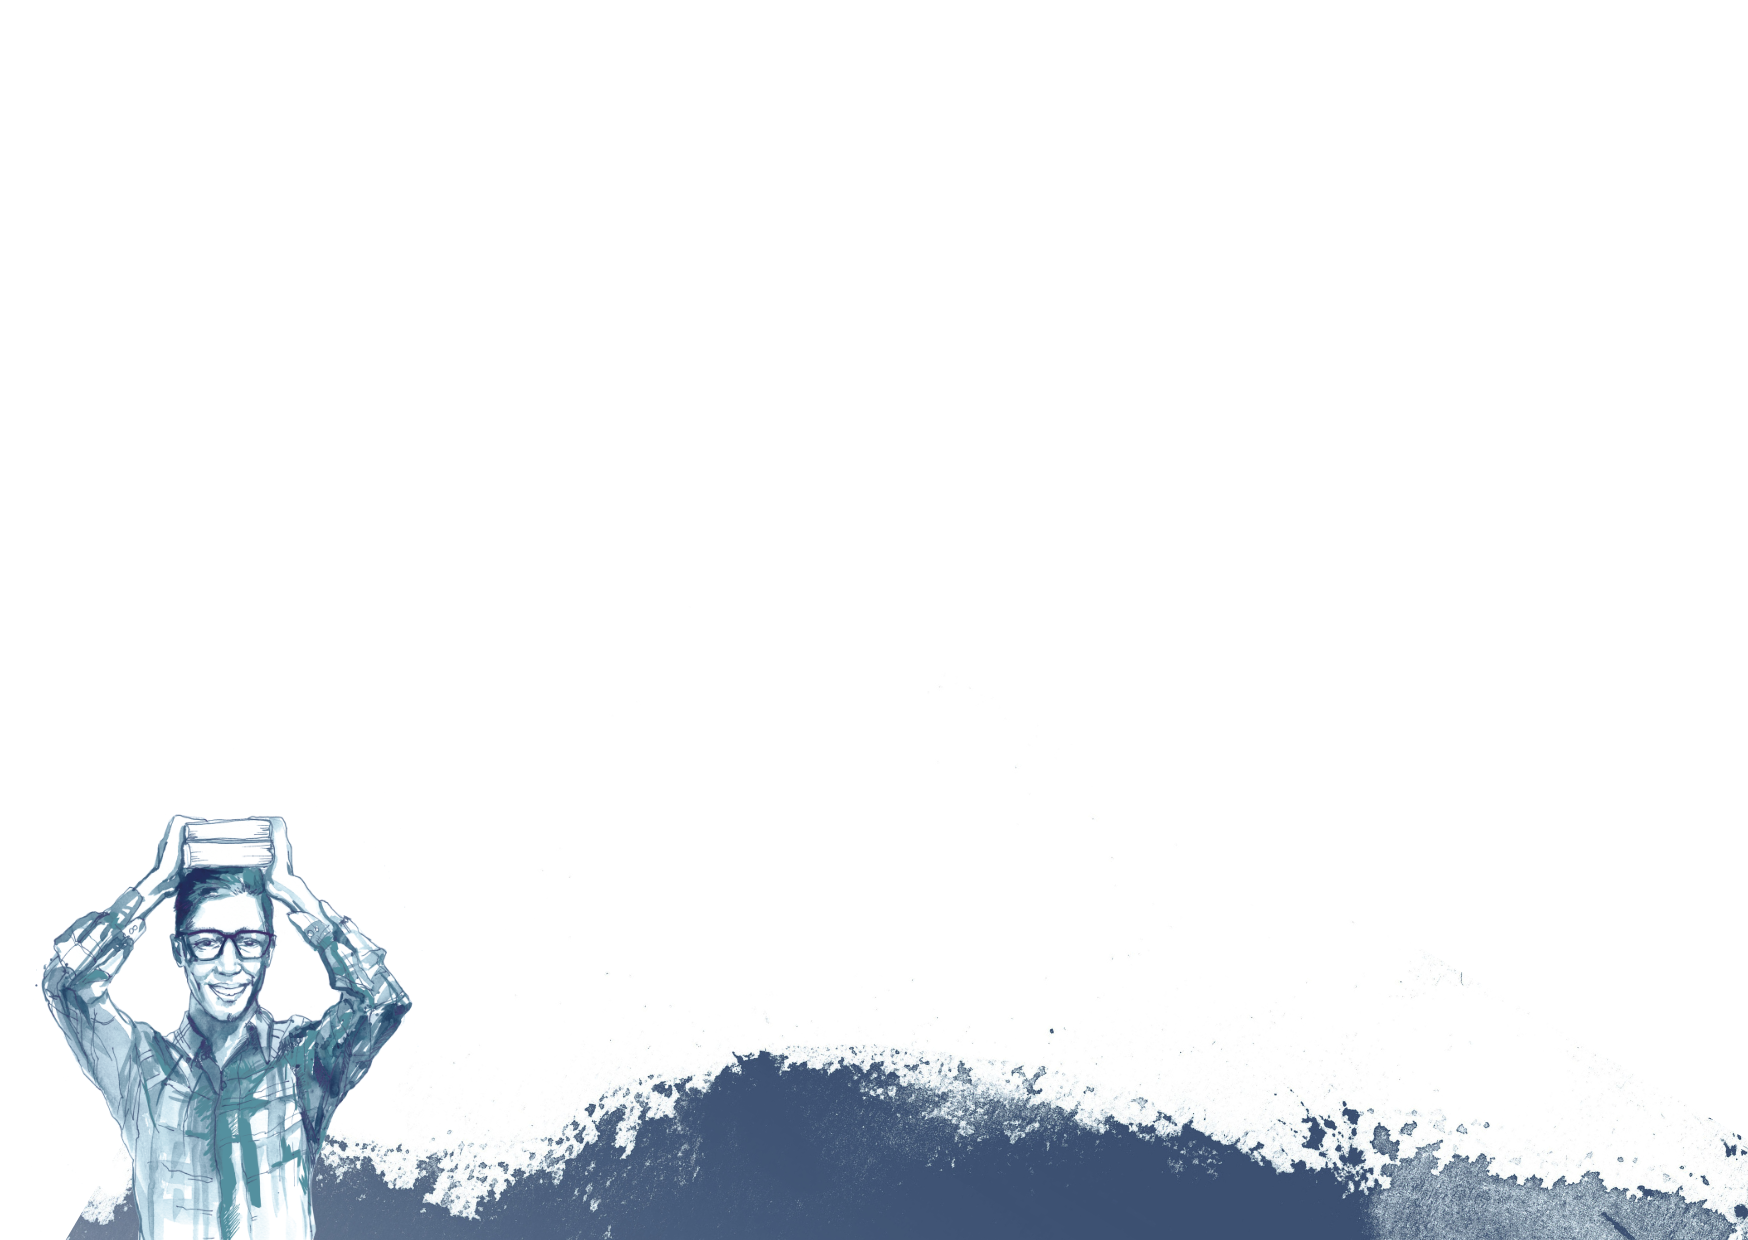
\includegraphics[width=\paperwidth,height=\paperheight]{Karteikarten Rückseite.png}}
]{mein.hintergrund.gerade}

% Jetzt fügen wir die Layer dem Stil hinzu, den du in deinen Umgebungen nutzt
\AddLayersToPageStyle{scrheadings}{mein.hintergrund.ungerade, mein.hintergrund.gerade}

% Sicherstellen, dass der Stil aktiv ist
\pagestyle{scrheadings}

% % % Schrift % % %
\usepackage{cmbright}			% Serifenlose Schrift

% % % Farben, Bilder, Graphiken, Tabellen, etc. % % %
\usepackage{xcolor}
\usepackage{graphicx}
\usepackage{diagbox}			% ermöglicht Diagonale in Tabelle		
\usepackage{tabularx}
	\newcolumntype{L}[1]{>{\raggedright\arraybackslash}p{#1}} 		% linksbündig mit Breitenangabe
	\newcolumntype{C}[1]{>{\centering\arraybackslash}p{#1}} 		% zentriert mit Breitenangabe
	\newcolumntype{R}[1]{>{\raggedleft\arraybackslash}p{#1}} 		% rechtsbündig mit Breitenangabe
\usepackage{fancybox}			% Rahmen mit \ovalbox{argument}

\usepackage{enumitem}			% Für Aufzählungen

% % % Vektorgraphiken mit TikZ % % %
\usepackage{tikz}
	% % % tikz-Bibliotheken
	\usetikzlibrary{
	               	backgrounds,
	               	calc,
	                intersections,
	                external
					}
\usepackage{tikz-3dplot} 		% Für die 3D-Schmankerl ;-)
	% % % Globale tikz-Einstellungen für Graphiken
	\tikzset{ 	asymptote/.style 		={	densely dashed,
											draw=black
											},
				funktionsgraph/.style	={	thick,
											draw=black,
											scale=1,
											domain=\xmin:\xmax,
											variable=\x,
											samples=200
											},
				gitter/.style			={	dotted,
											thin,
											draw=darkgray
											},
				integral/.style			={	fill=gray!50
											},
				tangente/.style			={	draw=black,
											densely dashed
											},
				kreis/.style			={	draw,circle,minimum size=2em,inner sep=1
											}
				}

% % % Mathematisches % % %
\usepackage{amsmath}          	% enthält nützliche Makros für Mathematik
\usepackage{amsfonts}         	% spezielle AMS-Mathematik-Fonts
\usepackage{amssymb}          	% spezielle AMS-Mathematik-Fonts
\usepackage{mathtools}			% nützliche Mathematikumgebungen
\usepackage{dsfont}           	% Zur Definition von Zahlmengen mit z.B. \mathds{R} für die Reellen Zahlen
\usepackage{nicefrac}			% alternative Darstellung für Brüche mit \nicefrac{3}{4}
\usepackage{icomma}				% Komma als Dezimaltrennzeichen
\usepackage{extarrows}
	
% % % Abkürzungen für Mengen % % % 
	\newcommand{\N}{\mathbb{N}}     % natürliche Zahlen
	\newcommand{\Z}{\mathbb{Z}}     % ganze Zahlen
	\newcommand{\Q}{\mathbb{Q}}     % rationale Zahlen
	\newcommand{\R}{\mathbb{R}}     % reelle Zahlen
	\newcommand{\C}{\mathbb{C}}     % komplexee Zahlen
	\newcommand{\D}{\mathbb{D}}     % Definitionsmenge
	\newcommand{\W}{\mathbb{W}}     % Wertemenge

% % % Abkürzungen Analysis % % %
	\newcommand{\euler}{\mathrm{e}}		% eulersche Zahl
	\newcommand{\abs}[1]{\ensuremath{\left\vert#1\right\vert}} %Große Betragsstriche
	\newcommand{\dx}{\,\mathrm{d}x}    	% dx beim Integral
	\newcommand{\FE}{\,\text{FE}}		% Flächeneinheiten
	\newcommand{\LE}{\,\text{LE}}		% Längeneinheiten
	\newcommand{\VE}{\,\text{VE}}		% Volumeneinheiten
	\newcommand{\gansgleich}{=} 		% Alternativ: Gleichheitszeichen mit Gänsefüßchen \stackrel{''}{=}
	\newcommand{\ohne}{\backslash} 	
	\newcommand{\lgans}{\hspace{-.25em}\raisebox{2ex}{"}\hspace{-.25em}}	% Linke Anführungszeichen beim Limes
	\newcommand{\rgans}{\hspace{-.25em}\raisebox{2ex}{"}\hspace{-.25em}}	% Rechte Anführungszeichen beim Limes

% % % Abkürzungen Stochastik % % %
	\newcommand{\erg}[1]{{\mathrm{#1}}}							% Ereignis
	\newcommand{\geg}[1]{\overline{\mathrm{#1}}}				% Gegenereignis
	\newcommand{\wkeit}[2][]{\mathrm{P}_{#1}\left(#2\right)}	% Wahrschinlichkeit 
	\DeclareMathOperator{\erw}{E}			% Erwartungswert
	\DeclareMathOperator{\var}{VAR}			% Varianz
\usepackage{upgreek}						% stellt aufrechte griechische Buchstaben bereit
	\newcommand{\std}{\upsigma}				% Standardabweichung
	\DeclareMathOperator{\bern}{B}			% Bernoulli
	% % % Umgebung für Vierfeldertafel
	\newenvironment{vierfelder}{
		\begin{center}
		\renewcommand{\arraystretch}{2}
		\begin{tabular}{C{1.25cm}|C{2cm}|C{2cm}|C{1.25cm}}
		}{
		\end{tabular}
		\end{center}}

% % % Abkürzungen Geometrie % % %
	\newcommand{\vektor}[1]{\left(\hspace{-1ex}\begin{array}{r}#1\end{array}\hspace{-1ex}\right)} 	% Kurzschreibweise, z.B. \vektor{1\\2\\3}
	\newcommand{\mal}{\circ}			% Zeichen für Skalarprodukt
\usepackage{array}				
	\newcolumntype{M}{>{{}}l<{{}}}		% Eigene Umgebung zur Ausrichtung von Gleichungssystemen
	\newenvironment{glsystem}{\arraycolsep=0pt\def\arraystretch{1.3}\array}{\endarray}
	% % % Siehe http://texwelt.de/wissen/fragen/421/wie-kann-man-in-mehrzeiligen-formelumgebungen-an-mehreren-stellen-ausrichten
	\newcommand{\I}{\mathrm{(I)}}		% manuelle Numerierung von Gleichungssystemen
	\newcommand{\II}{\mathrm{(II)}}		% manuelle Numerierung von Gleichungssystemen
	\newcommand{\III}{\mathrm{(III)}}	% manuelle Numerierung von Gleichungssystemen
\usepackage{esvect}					% Paket für Vektorpfeile, stellt \vv{} bereit
	\renewcommand{\vec}{\vv}		% Neudefinition des Befehls für Pfeile über Buchstaben


%\usepackage{showframe}					% Zeigt Seitenränder an (nützlich bei Wartungsarbeiten)

\begin{document}
\begin{frage}
	Karteikarten
\bigskip
	Mathematik
	\large
	
	\bigskip
	
	$\copyright$ AKADEMUS - Regensburg
\end{frage}
\begin{antwort}
	\copyright{} AKADEMUS
\end{antwort}
\begin{frage}
	Nullstellen einer Funktion?
	
\end{frage}
\begin{antwort}
	Ansatz: Funktion mit 0 gleichsetzen
	\[
	f(x)=0
	\]
\end{antwort}
\begin{frage}
	Nullstellen: Lineare Funktion
		
	z.B.: $f(x)=4x-12$
		
\end{frage}
\begin{antwort}
	Einfach umstellen:
	\[
	4x-12=0
	\]
	\[
	4x=12
	\]
	\[
	x=3
	\]
\end{antwort}
\begin{frage}
	Nullstellen: Quadratische Funktion
	\[
		f(x)=2x^2+6x-8
	\]
\end{frage}
\begin{antwort}
		\[
		2x^2+6x-8=0
		\]
	"`Mitternachtsformel"'
	\[
		x_{1,2}=\frac{-b\pm\sqrt{b^2-4ac}}{2a}
	\]
	\[
	x_{1,2}=\frac{-6\pm\sqrt{6^2-4\cdot2\cdot(-8)}}{2\cdot2 }
	\]
	\[
	x_{1}=1,\;x_{2}=-4
	\]

\end{antwort}
\begin{frage}
	Nullstellen: Funktion 3. Grades
	\[
	f(x)=2x^3+2x^2-24x
	\]
\end{frage}
\begin{antwort}
	\normalsize\begin{enumerate}
		\item Schritt: $x$ Ausklammern
		\item Schritt: Mitternachtsformel in der Klammer anwenden
	\end{enumerate}
	\normalsize\begin{align*}
		2x^3+2x^2-24x&=0\\
		x\cdot(2x^2+2x-24)&=0\\
		=>	x_{1}&= 0\\
		x_{2,3}&= ...Mitternachtsformel\\
		=>	x_{2}=3,\;x_{3}&=-4\\
	\end{align*}	
\end{antwort}
\begin{frage}
	Nullstellen: Gebrochene Funktion
	\[
	f(x)=\frac{4x-12}{x^2-4}
	\]
\end{frage}
\begin{antwort}
	Zähler mit 0 gleichsetzen:
	\[
	4x-12=0
	\]
	\[
	x=3
	\]
\end{antwort}
\begin{frage}
	Nullstellen: e-Funktion
	\[
	f(x)=(2x-4)\cdot{e^{3x+4}}
	\]
\end{frage}
\begin{antwort}
	"`e kann niemals 0 werden!"'
	\[
	{e^{3x+4}}\neq0
	\]
	"`Also kann nur der Faktor in der Klammer 0 werden!"'
	\[
	2x-4=0
	\]
	\[
	x=2
	\]
\end{antwort}
\begin{frage}
	Nullstellen: ln-Funktion
	\[
	f(x)=ln(2x-5)
	\]
\end{frage}
\begin{antwort}
	\begin{align*}
		ln(2x-5)&=0\\
		{e^{ln(2x-5)}}&=e^0\\
		2x-5&=1\\
		x&=3
	\end{align*}

\end{antwort}
\begin{frage}
	Definitionsmenge
\end{frage}
\begin{antwort}
	\begin{enumerate}
		\item Der Nenner muss ungleich 0 sein: $N \neq 0$
		\item Unter einer Wurzel müssen Werte größer oder gleich 0 sein: $\sqrt{\ge 0}$
		\item Im $ln$ muss immer etwas größeres als 0 stehen: $ln(>0)$\
	\end{enumerate}
\end{antwort}
\begin{frage}
	Definitionsmenge angeben:
	\begin{align*}
	     f_1(x)&=\frac{4x-12}{x-4} \\
		 f_2(x)&=\sqrt{2x-8}\\
		 f_3(x)&=ln(x+1)\\
	\end{align*}
\end{frage}
\begin{antwort}
	\begin{align*}
	   	  \D_{f_1}&=\R\big\backslash\big\{4\big\} \\
		  \D_{f_2}&=[4;\infty[ \\
		  \D_{f_3}&=]-1;\infty[ \\
	\end{align*}
\end{antwort}
\begin{frage}
	Wertemenge
\end{frage}
\begin{antwort}
	\begin{enumerate}
		\item Berechne die Grenzen an den Rändern des Definitionsbereichs: $\lim\limits_{x \rightarrow\pm\infty}{f(x)}$
		\item Berechne die Extrema inklusive y-Wert.
		\item Aus den in 1. und 2. errechneten Werten ergeben sich die Bereiche der Wertemenge.
	\end{enumerate}
\end{antwort}
\begin{frage}
	$x$-Achsenschnittpunkte
\end{frage}
\begin{antwort}
	\begin{enumerate}
		\item Setze $f(x)=0$ (für die Nullstellen)
		\item Löse Gleichung nach $x$ auf
		\item Schreibe die Ergebnisse als Punkte; z.B. N(7|0)
	\end{enumerate}
\end{antwort}
\begin{frage}
	$y$-Achsenschnittpunkt
\end{frage}
\begin{antwort}
	\begin{enumerate}
		\item $f(0)$ bestimmen; setze $0$ in $f(x)$ ein
		\item Schreibe das Ergebnis als Punkt; z.B. S(0|7)
	\end{enumerate}
\end{antwort}
\begin{frage}
	Achsensymmetrie zur y-Achse
\end{frage}
\begin{antwort}
	\LARGE	$f(x)=f(-x)$ 
\end{antwort}
\begin{frage}
	Punktsymmetrie zum Ursprung
\end{frage}
\begin{antwort}
	\LARGE	 $-f(x)=f(-x)$
\end{antwort}
\begin{frage}
	Gib je ein Beispiel für eine achsensymmetrische Funktion zur y-Achse und für eine punktsymmetrische Funktion zum Ursprung an.
\end{frage}
\begin{antwort}
	\begin{enumerate}
		\item Achsensymmetrisch zur y-Achse: $f(x)=x^2$
		\item Punktsymmetrisch zum Ursprung: $f(x)=x^3$
	\end{enumerate}
\end{antwort}
\begin{frage}
	Waagrechte Asymptoten
\end{frage}
\begin{antwort}
	\begin{enumerate} 
		\item Berechne $\lim\limits_{x \rightarrow \infty}{f(x)}$ und $\lim\limits_{x \rightarrow -\infty}{f(x)}$	
		
		\item Wenn eine Zahl rauskommt, dann lautet die waagrechte Asymptote y = \textbf{diese Zahl}
		
		\item Wenn $\infty$ oder  $-\infty$ rauskommt, gibt es keine waagrechten Asymptoten.
			
	\end{enumerate} 
\end{antwort}
\begin{frage}
	Senkrechte Asymptoten
	
\end{frage}
\begin{antwort}
	\begin{itemize} 
		\item \large Wo die Funktion Definitionslücken hat, hat sie ggf. auch senkrechte Asymptoten.		
		
		\item Allerdings muss der Limes bei den Definitionslücken gegen  $\pm\infty$ gehen. Also: 
		 $\lim\limits_{x \rightarrow \text{Def.Lücke}^+}{f(x)}=\pm\infty$ 
		 
		 und $\lim\limits_{x \rightarrow \text{Def.Lücke}^-}{f(x)}=\pm\infty$	
	
		\item senkrechte Asymptote: x= \textbf{Definitionslücke}
		
		
	\end{itemize} 
\end{antwort}
\begin{frage}
	Schräge Asymptoten \bigskip
	
	Bsp: $f(x)=2x -4 +\frac{3}{x+1}$
\end{frage}
\begin{antwort}
	\begin{itemize} 
		\item \large Wenn der Zählergrad einer gebrochen-rationalen Funktion genau um 1 größer ist als der Nennergrad, dann gibt es eine schräge Asymptote.		
		
		\item Die schräge Asymptote kann leicht ausgelesen werden, sobald man die Funktion in folgender Form gegeben hat: $f(x)=\textbf{ax+b} +\frac{\text{Bruch mit  Z{"a}hlergrad}}{<Nennergrad}$ 
		
		$\text{schräge Asymptote: } y=\textbf{ax+b}$	Im Beispiel: $\textbf {y=2x-4}$
		
		\textbf{Beachte:} \large Sollte die Funktion nicht in der benötigten Form gegeben sein, so muss mittels Polynomdivision die Funktion auf die benötigte Form gebracht werden.
		
		
	\end{itemize} 
\end{antwort}
\begin{frage}
	\LARGE Gib den Term einer gebrochen-rationalen Funktion an, die
	\begin{itemize} \large
		\item bei x=2 eine senkrechte Asymptote hat,		
		\item bei x=3 einen Pol ohne Vorzeichenwechsel hat, 
		\item bei x=4 einen Pol mit Vorzeichenwechsel hat,
		\item bei x=5 eine berührende Nullstelle hat,	
		\item bei x=6 ein behebbare Definitionslücke hat.	
		
	\end{itemize} 
	
\end{frage}
\begin{antwort}
	\LARGE $f(x)=\frac{ (x-5)^2 \cdot (x-6)}{(x-2) \cdot (x-3)^2 \cdot (x-4) \cdot (x-6)}$
\end{antwort}
\begin{frage}
	\LARGE Gib den Term einer gebrochen-rationalen Funktion an, die
	\begin{itemize} \large
		\item bei y=2 eine waagrechte Asymptote hat,		
		\item bei x=3 einen Pol mit Vorzeichenwechsel hat, 
		\item bei x=4 einen Pol ohne Vorzeichenwechsel hat.	
		
	\end{itemize} 
	
\end{frage}
\begin{antwort}
	\LARGE $f(x)=\frac{ 2x^3}{(x-3) \cdot (x-4)^2}$
\end{antwort}
\begin{frage}
	Verschiebung und Streckung von Funktionen  \bigskip
	
	$f(x)=a \cdot sin(b(x+c))+d$
\end{frage}
\begin{antwort}
	$f(x)=a \cdot sin(b(x+c))+d$
	\begin{itemize}
		\item a: Streckung in y-Richtung um den Faktor a
		\item b: Streckung in x-Richtung um den Faktor $\frac{1}{b}$
		\item c: Verschiebung um c in negative x-Richtung
		\item d: Verschiebung um d in positive y-Richtung
							
	\end{itemize}
	
	(Funktioniert auch bei allen anderen Funktionen)
\end{antwort}
\begin{frage}
	Wie geht die Funktion $f(x)=2 \cdot ln(x-3)+4$ aus der 
	Funktion $g(x)=ln(x)$ hervor?
\end{frage}
\begin{antwort}
	$f(x)=2 \cdot ln(x-3)+4$
	\begin{itemize}
		\item Streckung in y-Richtung um den Faktor 2		
		\item Verschiebung um 3 nach rechts
		\item Verschiebung um 4 nach oben							
	\end{itemize}	
\end{antwort}
\begin{frage}
	Ableitregel für Polynome
	
	z.B.: $f(x)=3x^4+2x^3-7$
	
\end{frage}
\begin{antwort}
	Ableitregel Polynome:
	\[
	f(x) = n \cdot x^m
	\]
	\[	
	f'(x)= nm \cdot x^{m-1}
	\]
	Im Beispiel:
	\[
	f'(x)=12x^3+6x^2
	\]
\end{antwort}
\begin{frage}
	Produktregel
	
	z.B.: $f(x)=sin(x)\cdot2x^3$
	
\end{frage}
\begin{antwort}
	Produktregel:
	\[
	f(x) = u(x)\cdot v(x)
	\]
	\[
	f'(x)=u'(x)\cdot v(x)+u(x)\cdot v'(x)
	\]
	Im Beispiel:
	\[
	f'(x)=cos(x)\cdot 2x^3 + sin(x)\cdot 6x^2
	\]
\end{antwort}
\begin{frage}
	Quotientenregel
	
	z.B.: $f(x)=\frac{sin(x)}{3x^2}$
	
\end{frage}
\begin{antwort}
	Quotientenregel:
	\normalsize
	\[
	\frac{NAZ-ZAN}{N^2}=\frac{Nenner \cdot AbleitungZ{"a}hler-Z{"a}hler \cdot AbleitungNenner}{Nenner^2}
	\]
	\Large
	Im Beispiel:
	\[
	f'(x)=\frac{3x^2 \cdot cos(x) - sin(x) \cdot (6x)}{(3x^2)^2}
	\]
\end{antwort}
\begin{frage}
	Kettenregel
	
	z.B.: $f(x)={sin(3x^2)}$
	
\end{frage}
\begin{antwort}
	Kettenregel:
	\[
	(f(g(x)))'=f'(g(x))\cdot g'(x)
	\]
	Im Beispiel:
	\[
	f'(x)=cos(3x^2)\cdot 6x
	\]
\end{antwort}
\begin{frage}
	Grenzwerte: $\lim\limits_{x \rightarrow \pm\infty}{f(x)}$
	\bigskip
	
	bei gebrochen-rationalen Funktionen
	
	(Tipp: 3 Möglichkeiten!)
	
\end{frage}
\begin{antwort}
	\large
	\[
	\lim\limits_{x \rightarrow \pm\infty}{\frac{4x^3 - 6x}{2x^2+4x-1}}=Z{"a}hlergrad>Nennergrad=\pm\infty^*
	\]
	\footnotesize 
	*Für das Vorzeichen: Jeweils +100 und -100 in f(x) einsetzen
	\large
	\[
	\lim\limits_{x \rightarrow \pm\infty}{\frac{5x^2+6x+4}{2x^4-6x}}=Z{"a}hlergrad<Nennergrad=0
	\]
	\[
	\lim\limits_{x \rightarrow \pm\infty}{\frac{\textbf{-2}x^3+4x}{\textbf{5}x^3 - 6x+1}}=Z{"a}hlergrad=Nennergrad=\frac{\textbf{-2}}{\textbf{5}}
	\]
\end{antwort}
\begin{frage}
	Bestimme die Gleichung der Tangente an der Stelle (z.B.) x=7
\end{frage}
\begin{antwort}
	\begin{enumerate}
		\item $m=f'(7)$
		\item $y=f(7)$
		\item $m$, $y$ und $x(=7)$ in $y= mx+t$ einsetzen und nach $t$ auflösen.
		\item Fertige Tangentengleichung $y= mx+t$ angeben. (Für y und x keine Zahlen einsetzen!)
		
	\end{enumerate}
\end{antwort}
\begin{frage}
	Umrechnung von Steigung und Winkel
\end{frage}
\begin{antwort}
	 $m=tan(\alpha)$
	 
	 $\alpha=tan^{-1}(m)$
\end{antwort}
\begin{frage}
	Gib ein Beispiel für eine Funktion an, die in $x=13$ nicht differenzierbar ist.
\end{frage}
\begin{antwort}
	$f(x)=|x-13|$
\end{antwort}

\begin{frage}
		Kurzcheckup's e-Funktion
		\begin{center}
				$e^0=$\\
				$e^{ln(13)}=$\\
				$e^\infty=$\\
				$e^{-\infty}=$				
		\end{center}
\end{frage}
\begin{antwort}
	\begin{center}
		$e^0=1$\\
		$e^{ln(13)}=13$\\
		$e^\infty=\infty$\\
		$e^{-\infty}=0$				
	\end{center}
\end{antwort}
\begin{frage}
	Kurzcheckup's ln-Funktion
	\begin{enumerate}
		\item $ln(1)=$
		\item $ln(e)=$
		\item $ln(\infty)=$
		\item $ln(e^{13})=$				
	\end{enumerate}
\end{frage}
\begin{antwort}
	\begin{enumerate}
		\item $ln(1)=0$
		\item $ln(e)=1$
		\item $ln(\infty)=\infty$
		\item $ln(e^{13})=13$					
	\end{enumerate}
\end{antwort}
\begin{frage}
	Extrema und Monotonie \bigskip 
	
	(6 Schritte)	
\end{frage}

\begin{antwort}
	\begin{enumerate}
		\item $f'(x)$ bestimmen
		\item Nullstellen der 1. Ableitung (= Extremstellen)
		\item y-Werte bestimmen (in f(x) einsetzen)
		\item Monotonietabelle angeben
		\item Hoch-, Tief- und Terrassenpunkte angeben
		\item Monotonieintervalle angeben						
	\end{enumerate}
\end{antwort}

\begin{frage}
	Wendepunkte und Krümmung \bigskip 
	
	(6 Schritte)	
\end{frage}
\begin{antwort}
	\begin{enumerate}
		\item $f''(x)$ bestimmen
		\item Nullstellen der 2. Ableitung (= Wendestellen)
		\item y-Werte bestimmen (in f(x) einsetzen)
		\item Krümmungstabelle angeben
		\item Wendepunkte angeben
		\item Krümmungsintervalle angeben						
	\end{enumerate}
\end{antwort}
\begin{frage}
	Zusammenhänge zwischen f(x) und f'(x)	
	
	(Nützlich für das Zeichnen von Ableitungen und Stammfunktionen)
\end{frage}
\begin{antwort}
	\begin{tikzpicture}[scale=2]
	\draw (0,-0.1) -- (0,2.8);
	\draw (-3,2.6) -- (3,2.6) ;
	\draw (-1,3) node[below left]{$f(x)$}  (1,3) node[below right]{$f'(x)$} ;	
	\draw (-0.5,2.5) node[below left]{Extrempunkt} (0.5,2.5) node[below right]{Nullstelle} ;
	\draw (-0.5,2) node[below left]{Wendepunkt} (0.5,2) node[below right]{Extrempunkt} ;
	\draw (-0.5,1.5) node[below left]{monoton steigend} (0.5,1.5) node[below right]{überhalb x-Achse};
	\draw (-0.5,1) node[below left]{monoton fallend} (0.5,1) node[below right]{unterhalb x-Achse};
	\draw (-0.5,0.5) node[below left]{Grad d. Fkt.} (0.5,0.5) node[below right]{Grad-1 d. Fkt.};
	\draw (-0.5,0.25) node[below left]{(z.B. Parabel)} (0.5,0.25) node[below right]{(Gerade)};
	\end{tikzpicture}		

\end{antwort}	
\begin{frage}
	Zusammenhänge zwischen f(x) und f'(x) Teil 2
	
	(Nützlich für das Zeichnen von Ableitungen und Stammfunktionen)
\end{frage}
\begin{antwort}
	\begin{tikzpicture}[scale=2]
	\draw (0,0.2) -- (0,2.8);
	\draw (-3,2.6) -- (3,2.6) ;
	\draw (-1,3) node[below left]{$f(x)$}  (1,3) node[below right]{$f'(x)$} ;	
	\draw (-0.5,2.5) node[below left]{\large waagrechte Asympt.} (0.5,2.5) node[below right]{\large waagrechte Asympt.} ;
	\draw (-0.5,2.25) node[below left]{} (0.5,2.25) node[below right]{\normalsize (bei y=0)};
	\draw (-0.5,1.75) node[below left]{\large senkrechte Asympt.} (0.5,1.75) node[below right]{\large senkrechte Asympt.} ;
	\draw (-0.5,1.5) node[below left]{} (0.5,1.5) node[below right]{\normalsize (an gleicher Stelle)};
	\draw (-0.5,1) node[below left]{\large schräge Asympt.} (0.5,1) node[below right]{\large waagrechte Asympt.} ;
	\draw (-0.5,0.75) node[below left]{} (0.5,0.75) node[below right]{\normalsize (bei y=Steigung der} ;
	\draw (-0.5,0.6) node[below left]{} (0.6,0.55) node[below right]{\normalsize schrägen Asymptote)} ;

	\end{tikzpicture}			
	
\end{antwort}			
\begin{frage}
	Fläche zwischen $f(x)$ und der x-Achse
\end{frage}

\begin{antwort}
	\begin{enumerate} 
		\item Nullstellen berechnen: $f(x)=0$
		
		Man erhält die Integrationsgrenzen $x_{klein}$ und $x_{gro{"s}}$.
		\item Fläche berechnen: 
		$A=\abs{\displaystyle\int\limits_{x_{klein}}^{x_{gro{"s}}} \! f(x) \, \mathrm{d}x}$
		
		\textbf{Beachte:} \Large Wenn 3 Nullstellen statt 2 existieren, muss das Integral aufgeteilt werden:
		
		$A=\abs{\displaystyle\int\limits_{x_{klein}}^{x_{mittel}} \! f(x) \, \mathrm{d}x}+\abs{\displaystyle\int\limits_{x_{mittel}}^{x_{gro{"s}}} \! f(x) \, \mathrm{d}x}$
	\end{enumerate} 
\end{antwort}

\begin{frage}
	Fläche zwischen zwei Funktionen $f(x)$ und $g(x)$
\end{frage}
\begin{antwort}
		\begin{enumerate} 
			\item Schnittstellen berechnen: $f(x)=g(x)$
			
			Man erhält die Integrationsgrenzen $x_{klein}$ und $x_{gro{"s}}$.
			\item Fläche berechnen: 
				$A=\abs{\displaystyle\int\limits_{x_{klein}}^{x_{gro{"s}}} \! (f(x)-g(x)) \, \mathrm{d}x}$
			
			\textbf{Beachte:} \Large Wenn 3 Schnittstellen statt 2 existieren, muss das Integral aufgeteilt werden:
			
				$\abs{\displaystyle\int\limits_{x_{klein}}^{x_{mittel}} \! (f(x)-g(x)) \, \mathrm{d}x}+\abs{\displaystyle\int\limits_{x_{mittel}}^{x_{gro{"s}}} \! (f(x)-g(x)) \, \mathrm{d}x}$
		\end{enumerate} 
\end{antwort}
\begin{frage}
	Integrale im Sachzusammenhang (also bei Anwendungsaufgaben) deuten
\end{frage}
\begin{antwort}
	Änderung pro Zeit $\xlongrightarrow{\text{Integrieren}}$ Gesamtänderung 
	
	\bigskip Beispiele
	
	\large\bigskip
	Schadstoffausstoß pro Minute $\xlongrightarrow{\text{Integrieren}}$ Gesamtausstoß
	Rohrdurchfluss pro Minute $\xlongrightarrow{\text{Integrieren}}$ Gesamte Wassermenge
\end{antwort}
\begin{frage}
	Geometrische Interpretation der Vorzeichen von Integralen.
\end{frage}
\begin{antwort}
	\begin{itemize} 
		\item Ergebnis ist positiv: Der Flächenanteil oberhalb der x-Achse ist größer als unterhalb der x-Achse.
		\item Ergebnis ist 0: Der Flächenanteil oberhalb und unterhalb der x-Achse ist gleich groß.
		\item Ergebnis ist negativ: Der Flächenanteil unterhalb der x-Achse ist größer als oberhalb der x-Achse.
	\end{itemize}
\end{antwort}
\begin{frage}
	Die Integralfunktion
\end{frage}
\begin{antwort}
	\begin{itemize}
		\item $F_a(x)=\displaystyle\int\limits_{a}^{x} \! f(t) \, \mathrm{d}t$
		\item a ist immer eine Nullstelle der Integralfunktion
		\item Deutung: Die Integralfunktion gibt die Flächenbilanz zwischen $f(x)$ und der $x$-Achse von der Nullstelle $a$ bis zu einem beliebigen Wert $x$ an.		
	\end{itemize}
\end{antwort}
\begin{frage}
	Zeige, dass $F(x)$ eine Stammfunktion zu $f(x)$ ist
\end{frage}
\begin{antwort}
	Einfach $F(x)$ ableiten. 
	
	Es muss also gelten: F'(x)=f(x)
\end{antwort}
\begin{frage}
	Bilde folgende Stammfunktionen: 
	\flushleft 
	$f_1(x)=6x^2+4x-7$
	
	\bigskip
   	$f_2(x)=cos(x)$
   	
   	\bigskip
	$f_3(x)=sin(x)$	
\end{frage}
\begin{antwort}
	\flushleft
	$f_1(x)=6x^2+4x-7 \longrightarrow F_1(x)=2x^3+2x^2-7x+c$ 

	\bigskip
	$f_2(x)=cos(x) \longrightarrow F_2(x)=sin(x)+c$
	
	\bigskip	
    $f_3(x)=sin(x) \longrightarrow F_3(x)=-cos(x)+c$
	
\end{antwort}
\begin{frage}
	Bilde folgende Stammfunktionen: 
	\flushleft 
	$f_1(x)=\frac{1}{x}$
	
	\bigskip
	$f_2(x)=\frac{5}{x}$
	
	\bigskip
	$f_3(x)=\frac{1}{x^3}$	
\end{frage}
\begin{antwort}
	\flushleft
	$f_1(x)=\frac{1}{x} \longrightarrow F_1(x)=ln|x|+c$ 
	
	\bigskip
	$f_2(x)=\frac{5}{x}=5\cdot\frac{1}{x}  \longrightarrow F_2(x)=5\cdot ln|x|+c$ 
	
	\bigskip	
	$f_3(x)=\frac{1}{x^3}=x^{-3} \longrightarrow F_3(x)=-0,5x^{-2}+c$
	
\end{antwort}
\begin{frage}
	Bilde folgende Stammfunktionen: 
	\flushleft 
	$f_1(x)=\frac{6x^2-4}{2x^3-4x}$
	
	\bigskip
	$f_2(x)=\sqrt{x}$
	
	\bigskip
	$f_3(x)=\frac{2x^3-4x^2+4x}{2x^2}$	
\end{frage}
\begin{antwort}
	\flushleft
	$f_1(x)=\frac{6x^2-4}{2x^3-4x} \longrightarrow F_1(x)=ln|2x^3-4x|+c$ 
	
	\bigskip
	$f_2(x)=\sqrt{x}=x^{0,5} \longrightarrow F_2(x)=\frac{1}{1,5}x^{1,5}+c$
	
	\bigskip	
	$f_3(x)=\frac{2x^3-4x^2+4x}{2x^2}=\frac{2x^3}{2x^2}-\frac{4x^2}{2x^2}+\frac{4x}{2x^2}=x-2+\frac{2}{x} \longrightarrow F_3(x)=0,5x^2-2x+2ln|x|+c$	
\end{antwort}
\begin{frage}
	Bilde folgende Stammfunktionen: 
	\flushleft 
	$f_1(x)=\frac{2x-4}{2x^2-8x}$
	
	\bigskip
	$f_2(x)=\sqrt{7x-1}$
	
	\bigskip
	$f_3(x)=sin(4x+2)$	
\end{frage}
\begin{antwort}
	\flushleft
	$f_1(x)=\frac{2x-4}{2x^2-8x}=\frac{1}{2}\cdot\frac{4x-8}{2x^2-8x}$
	
    $\longrightarrow F_1(x)=\frac{1}{2}\cdot ln|2x^2-8x|+c$ 
	
	\bigskip
	$f_2(x)=\sqrt{7x-1}=(\textbf{7}x-1)^{0,5}$
	
	$\longrightarrow F_2(x)=\frac{1}{1,5}(\textbf{7}x-1)^{1,5}\cdot\frac{1}{\textbf{7}}+c$
	
	\bigskip	
	$f_3(x)=sin(\textbf{4}x+2)$
	$\longrightarrow F_3(x)=-cos(\textbf{4}x+2)\cdot\frac{1}{\textbf{4}}+c$	
\end{antwort}
\begin{frage}
	Stammfunktion von Brüchen
	
	(2 Fälle!)
\end{frage}
\begin{antwort}
\normalsize\begin{itemize}
	\item Im Zähler steht die Ableitung vom Nenner:
	
	$\displaystyle\int \! \frac{g'(x)}{\textbf{g(x)}} \, \mathrm{d}x=ln|\textbf{g(x)}|+c$
	
	z.B.: $\displaystyle\int \! \frac{4x-6}{{2x^2-6x}} \, \mathrm{d}x=ln|{2x^2-6x}|+c$
	\item Es gibt nur einen Ausdruck mit '$n \cdot x^m$' im Nenner:
	
	 z.B.: $\displaystyle\int \! \frac{4x^3+x-2}{{x^2}} \, \mathrm{d}x=\displaystyle\int \! (\frac{4x^3}{{x^2}}+\frac{x}{{x^2}}-\frac{2}{{x^2}}) \, \mathrm{d}x$
	 
	 $=\displaystyle\int \! (4x+\frac{1}{{x}}-\frac{2}{{x^2}}) \, \mathrm{d}x=\displaystyle 2x^2+ln|x|+2x^{-1}+c$
	\end{itemize}
\end{antwort}
\begin{frage}
	Pfadregeln bei Baumdiagrammen
	
	(Bsp.: 3-maliger Münzwurf)
\end{frage}
\begin{antwort}
	\normalsize\begin{itemize}
		\item Entlang eines Astes multiplizieren, um eine ganz bestimmte Wahrscheinlichkeit auszurechnen.
				
		z.B.: Kopf, Kopf, Zahl: P(K;K;Z)
		\item Zwischen den Ästen addieren, um die Wahrscheinlichkeit eines Ereignisses mit mehreren Versuchsausgängen zu berechnen:
		
		z.B.: Zweimal Kopf, einmal Zahl: P(K;K;Z)+P(K;Z;K)+P(Z;K;K)
	\end{itemize}
\end{antwort}
\begin{frage}
	Baumdiagramm oder Vierfeldertafel
\end{frage}
\begin{antwort}
	\begin{itemize}
		\item Baumdiagramm: Bedingte Wahrscheinlichkeiten $P_B(A)$
		
		\item Vierfeldertafel: 
		
		Absolute Häufigkeiten (z.B.: 96 Schüler), Schnitt-Wahrscheinlichkeiten $P(A\cap B)$
	\end{itemize}
\end{antwort}
\begin{frage}
	Wahrscheinlichkeit, dass A oder B eintritt: 
	
	$P(A\bigcup B)$
\end{frage}
\begin{antwort}
	Satz von Sylvester:
	
	$P(A\bigcup B)=P(A)+P(B)- P(A\cap B)$
\end{antwort}
\begin{frage}
	Wahrscheinlichkeit, dass entweder A oder B eintritt: 
	
\end{frage}
\begin{antwort}
	$P(\text{entweder A oder B})=P(A)+P(B)- 2 \cdot P(A\cap B)$
\end{antwort}
\begin{frage}
	Stochastische Unabhängigkeit 
	
\end{frage}
\begin{antwort}
	$P(A\cap B)=P(A)\cdot P(B) \rightarrow$ Unabhängig
	
	
	$\hspace{2cm}\neq \hspace{3.5cm}    \rightarrow$ Abhängig
\end{antwort}
\begin{frage}
	Bedingte Wahrscheinlichkeit
	
\end{frage}
\begin{antwort}
	\LARGE
	$P_B(A)=\frac{P(A \text{ }\cap \text{ }B)}{P(B)}$
	\large
	\begin{itemize}
		\item Die Bedingung steht immer im Nenner
		\item Die Wahrscheinlichkeiten können dem Baumdiagramm bzw. der Vierfeldertafel
		entnommen werden.
	\end{itemize}
	
	
\end{antwort}
\begin{frage}
	Bernoulli-Formel
	
\end{frage}
\begin{antwort}
	\LARGE
	$P(X=k)=\binom{n}{k} \cdot p^k \cdot (1-p)^{n-k}$
	\large
	\begin{itemize}
		\item n = Anzahl Versuche
		\item k = Anzahl Treffer
		\item p = Trefferwahrscheinlichkeit
	\end{itemize}	
\end{antwort}
\begin{frage}
	Woran erkennt man ein Bernoulli-Experiment?
	
\end{frage}
\begin{antwort}
	Es gibt Treffer und Nieten; Experiment mit Zurücklegen.
	
	z.B.: 10 Schuss auf eine Klappscheibe mit Trefferquote 60 $\%$.
\end{antwort}
\begin{frage}
	\large
	Ein Schütze trifft sein Ziel mit p=0,6 und gibt 100 Schuss ab. Mit welcher Wahrscheinlichkeit trifft er 
	
	\LARGE 
	genau 17 mal?
	
\end{frage}
\begin{antwort}
	n=100, k=17, p=0,6
	
	\bigskip
	$P^{100}_{0,6}(X=17)=\binom{100}{17} \cdot 0,6^{17} \cdot (1-0,6)^{83}$
	
\end{antwort}
\begin{frage}
	\large
	Ein Schütze trifft sein Ziel mit p=0,6 und gibt 100 Schuss ab. Mit welcher Wahrscheinlichkeit trifft er 
	
	\LARGE 
	höchstens 20 mal?
	
\end{frage}
\begin{antwort}
	n=100, k$\leq$20, p=0,6
	
	\bigskip
	$P^{100}_{0,6}(X\leq 20)$
	
	(Tafelwerk!)
	
\end{antwort}
\begin{frage}
	\large
	Ein Schütze trifft sein Ziel mit p=0,6 und gibt 100 Schuss ab. Mit welcher Wahrscheinlichkeit trifft er 
	
	\LARGE 
	weniger als 20 mal?
	
\end{frage}
\begin{antwort}
	n=100, k<20, p=0,6
	
	\bigskip
	$P^{100}_{0,6}(X<20)=P^{100}_{0,6}(X\leq19)$
	
	(Tafelwerk!)
	
\end{antwort}
\begin{frage}
	\large
	Ein Schütze trifft sein Ziel mit p=0,6 und gibt 100 Schuss ab. Mit welcher Wahrscheinlichkeit trifft er 
	
	\LARGE 
	mindestens 20 mal?
	
\end{frage}
\begin{antwort}
	n=100, k$\geq$20, p=0,6
	
	\bigskip
	$P^{100}_{0,6}(X\geq 20)=1-P^{100}_{0,6}(X\leq 19)$
	
	 (Tafelwerk!)
	
\end{antwort}
\begin{frage}
	\large
	Ein Schütze trifft sein Ziel mit p=0,6 und gibt 100 Schuss ab. Mit welcher Wahrscheinlichkeit trifft er 
	
	\LARGE 
	mehr als 20 mal?
	
\end{frage}
\begin{antwort}
	n=100, k>20, p=0,6
	
	\bigskip
	$P^{100}_{0,6}(X>20)=1-P^{100}_{0,6}(X\leq 20)$
	
	(Tafelwerk!)
	
\end{antwort}
\begin{frage}
	\large
	Ein Schütze trifft sein Ziel mit p=0,6 und gibt 100 Schuss ab. Mit welcher Wahrscheinlichkeit trifft er 
	
	\LARGE 
	mindestens 20 mal aber höchstens 30 mal?
	
\end{frage}
\begin{antwort}
	n=100, 20$\leq$k$\leq$30, p=0,6
	
	\bigskip\large
	$P^{100}_{0,6}(20\leq X \leq30)=P^{100}_{0,6}(X\leq30)-P^{100}_{0,6}(X\leq19)$
	
	(Tafelwerk!)
	
\end{antwort}
\begin{frage}
	\large
	Ein Schütze trifft sein Ziel mit p=0,6. Mit welcher Wahrscheinlichkeit ist 
	
	\LARGE 
	der 20. Versuch der 6. Treffer?
	
\end{frage}
\begin{antwort}
	5 Treffer in den ersten 19 Versuchen und (=mal) ein Treffer beim 20. Versuch:
	
	n=19, k=5, p=0,6 und (=mal) n=1, k=1, p=0,6
	
	\bigskip
	$\binom{19}{5} \cdot 0,6^{5} \cdot (1-0,6)^{14} \hspace*{0.5cm}\cdot\hspace*{0.5cm} \binom{1}{1} \cdot 0,6^{1} \cdot (1-0,6)^{0}$
		
\end{antwort}
\begin{frage}
	\large
	Ein Schütze trifft sein Ziel mit p=0,6 und gibt 20 Schuss ab. Mit welcher Wahrscheinlichkeit trifft er  
	
	\LARGE 
	6 mal, jedoch nicht in den ersten 10 Versuchen?
	
\end{frage}
\begin{antwort}
	0 Treffer in den ersten 10 Versuchen und (=mal) 6 Treffer in den letzten 10 Versuchen:
	
	n=10, k=0, p=0,6 und (=mal) n=10, k=6, p=0,6
	
	\bigskip
	$\binom{10}{0} \cdot 0,6^{0} \cdot (1-0,6)^{10} \hspace*{0.5cm}\cdot\hspace*{0.5cm} \binom{10}{6} \cdot 0,6^{6} \cdot (1-0,6)^{4}$
	
\end{antwort}
\begin{frage}
	\large
	Ein Schütze trifft sein Ziel mit p=0,6 und gibt 20 Schuss ab. Mit welcher Wahrscheinlichkeit trifft er 
	
	\LARGE 
	genau 3 mal aber aufeinanderfolgend?
	
\end{frage}
\begin{antwort}
	n=20, k=3, p=0,6
	
	\bigskip
	$P(\text{k Treffer aufeinanderfolgend})=(n-k+1)\cdot p^{k} \cdot (1-p)^{n-k}$
	
	$P(\text{3 Treffer aufeinanderfolgend})=18\cdot 0,6^{3} \cdot (1-0,6)^{17}$
	
\end{antwort}
\begin{frage}
	Die 3-mindestens-Aufgabe
	
\end{frage}
\begin{antwort}
	\begin{enumerate}
		\item Erkennt man an den 3 'Mindestens' im Text. 
		\item Verwende folgende Formel:
		
		 $1-(1-p_{Treffer})^n\geq \alpha$
		\item Löse mittels $ln$ nach  n auf.
		\item Ergebnis immer aufrunden.
	\end{enumerate}
	
\end{antwort}
\begin{frage}
	Ziehen ohne Zurücklegen
	
\end{frage}
\begin{antwort}
	\LARGE
	 $p=\frac{\binom{SORTE1}{sorte1}\binom{SORTE2}{sorte2}}{\binom{\text{Wieviele gibt es ingesamt?}}{\text{Wieviele ziehe ich ingesamt?}}}$
	
\end{antwort}
\begin{frage}
	Wahrscheinlichkeitsverteilung
	
\end{frage}
\begin{antwort}
	\begin{itemize}
		\item Ist unabdingbar um Erwartungswerte und Varianzen zu berechnen. 
		\item Oben stehen die einzelnen Fälle $x_i$
		\item Unten stehen die zugehörigen Wahrscheinlichkeiten $P(X=x_i)$
		\item Die Wahrscheinlichkeiten unten müssen in der Summe immer 1 ergeben.
	\end{itemize}	
\end{antwort}	
\begin{frage}
	Erwartungswert
	
\end{frage}
\begin{antwort}
	\begin{itemize}
		\item Ist der durchschnittliche Ausgang eines Zufallsexperiments.
		Z.B. Gewinn pro Spiel 
		\item $E(X)=\mu=x_1 \cdot p_1 + x_2 \cdot p_2 + ...$
		\item Ausnahme Bernoulli: $\mu=n \cdot p$
		\item Ein Spiel ist fair, wenn der Erwartungswert 0 ist.
	\end{itemize}	
\end{antwort}	
\begin{frage}
	Varianz
	
\end{frage}
\begin{antwort}
	\begin{itemize}
		\item $Var(X)=(x_1-\mu)^2 \cdot p_1+(x_2-\mu)^2 \cdot p_2+...$		
		\item Ausnahme Bernoulli: $Var(X)=n \cdot p \cdot (1-p)$	
	\end{itemize}	
\end{antwort}	
\begin{frage}
	Standardabweichung
	
\end{frage}
\begin{antwort}
	\begin{itemize}
		\item Gibt die durchschnittliche Abweichung vom Erwartungswert an.		
		\item $\sigma=\sqrt{Var(X)}$	
	\end{itemize}	
\end{antwort}	
\begin{frage}
	Schema für Hypothesentest
	
\end{frage}
\begin{antwort}
	\begin{enumerate}
		\item Zahlenstrahl und Nullhypothese $H_0$ angeben
		
		=> Annahme- und Ablehnungsbereich  ($A \text{ bzw. }\overline{A}$)	
		\item $H_0$ angenommen oder abgelehnt?
		
		(Indem man  $\alpha \text{ bzw. }\beta$-Fehler rausfindet) 	
		\item In Lückenformel einsetzen: 
		
		$\alpha \text{ bzw. }\beta=P^n_p(A\text{ bzw. }\overline{A}\text{ (je nach 2.) })$	
	\end{enumerate}
	
\end{antwort}	
\begin{frage}
	Schema für Signifikanztest
	
\end{frage}
\begin{antwort}
	\begin{enumerate}
		\item Signifikanzniveau ist der $\alpha$-Fehler.
		\item Zahlenstrahl und Nullhypothese $H_0$ angeben
		
		=> Annahme- und Ablehnungsbereich  ($A \text{ bzw. }\overline{A}$)			
			
		\item In Lückenformel einsetzen: $P^n_p(\overline{A})\leq\alpha$	
	\end{enumerate}	
\end{antwort}	
\begin{frage}
	Signifikanzniveau
	
\end{frage}
\begin{antwort}
	\begin{itemize}
		\item Die Nullhypothese $H_0$ ist wahr, wird jedoch abgelehnt.
		\item Andere Bezeichnungen: 
		
		Fehler 1. Art oder $\alpha$-Fehler.	
	\end{itemize}	
\end{antwort}
\begin{frage}
	Fehler 2. Art
	
\end{frage}
\begin{antwort}
	\begin{itemize}
		\item Die Nullhypothese $H_0$ ist falsch, wird jedoch angenommen.
		\item Andere Bezeichnung: $\beta$-Fehler.	
	\end{itemize}	
\end{antwort}	
\begin{frage}
	Die Nullhypothese wird immer so aufgestellt, dass ...
	
\end{frage}
\begin{antwort}
	sie das Gegenteil des Ziels ist. Möchte man z.B. zeigen, dass p mehr als 40 $\%$ ist,
	so muss $H_0: p \le 40$ $\%$ sein.
	
	Ausnahme: Im Text steht, dass es sich hierbei um die Nullhypothese handelt.
\end{antwort}	
\begin{frage}
	\LARGE
	In einer Kiste sind 10 rote, 4 gelbe und 6 grüne Äpfel. Man entnimmt der Kiste 6 Äpfel. Wie viele Möglichkeiten gibt es, 3 rote, 2 gelbe und 1 grünen Apfel zu ziehen. 
	
\end{frage}
\begin{antwort}
	\LARGE
	$\binom{10}{3} \cdot \binom{4}{2} \cdot \binom{6}{1}$
\end{antwort}	
\begin{frage}
	\LARGE
	Wie viele Möglichkeiten gibt es, 5 Personen 
	
	\hspace{0.3cm}a) in ein Auto mit 5 Sitzplätzen zu setzen?
	
	\hspace{-0.25cm}b) in einen Kleinbus mit 7 Sitzplätzen zu setzen?
	
\end{frage}
\begin{antwort}
	\LARGE
	\hspace{1.3cm}	a) $5 \cdot 4 \cdot 3\cdot 2 \cdot 1=5!$
	
	b) $7 \cdot 6 \cdot 5\cdot 4 \cdot 3$
\end{antwort}	
\begin{frage}
	\LARGE
	Wie viele Möglichkeiten gibt es, 5 Personen aus einer Gruppe von 12 Personen auszuwählen, wenn
	es auf die Reihenfolge ankommt?
\end{frage}
\begin{antwort}
	\LARGE
	$\binom{12}{5} \cdot 5!$
\end{antwort}	
\begin{frage}
	Vektor von $A(1|2|-3)$ nach $B(3|-5|1)$ aufstellen
\end{frage}
\begin{antwort}
	Spitze minus Fuß:
	
	\bigskip		
		$\vec{AB}=\vec{B}-\vec{A}=\left(\begin{array}{c} 3-1 \\ -5-2 \\ 1+3\end{array} \right)=\left(\begin{array}{c} 2 \\ -7 \\ 4\end{array} \right)$
		
\end{antwort}		
\begin{frage}
	Länge eines Vektors
	
	Bsp.: $\vec{a}=\left(\begin{array}{c} 2 \\ 1 \\ -2\end{array} \right)$
\end{frage}
\begin{antwort}
	Formel: $\left|\vec{a}\right|=\sqrt{a_1^2 + a_2^2 + a_3^2}$
	
	\bigskip		
$\left|\vec{a}\right|=\left|\left(\begin{array}{c} 2 \\ 1 \\ -2\end{array} \right)\right|=\sqrt{2^2 + 1^2 + (-2)^2}=3$
	
\end{antwort}	
\begin{frage}
	\LARGE
	Prüfe, ob $\vec{a}=\left(\begin{array}{c} 3 \\ 2 \\ -4\end{array} \right)$ und  $\vec{b}=\left(\begin{array}{c} 4 \\ 0 \\ 3\end{array} \right)$ 
	senkrecht aufeinander stehen.
\end{frage}
\begin{antwort}
	
	$\left(\begin{array}{c} 3 \\ 2 \\ -4\end{array} \right) \circ \left(\begin{array}{c} 4 \\ 0 \\ 3\end{array} \right)= 3 \cdot 4 + 2 \cdot 0 -4\cdot 3=0$
	
	$=> \vec{a} \perp \vec{b}$
	
\end{antwort}	
\begin{frage}
	\LARGE
	Prüfe, ob $\vec{a}$ und  $\vec{b}$ 
	parallel zueinander sind.
\end{frage}
\begin{antwort}
	
	Mann muss prüfen, ob $\vec{a}$ und  $\vec{b}$ Vielfache sind!
	\begin{enumerate}
		\item Schreibe $k \cdot \vec{a}= \vec{b}$
		\item Rechne in allen drei Zeilen k aus.			
		\item Wenn in allen drei Zeilen das gleiche k rauskommt, sind $\vec{a}$ und $\vec{b}$
		parallel, bzw. Vielfache, bzw. linear abhängig.	
	\end{enumerate}	
	
\end{antwort}	
\begin{frage}

	Berechne  $\left(\begin{array}{c} 2 \\ 3 \\ 4\end{array} \right) \times \left(\begin{array}{c} -5 \\ 0 \\ 1\end{array} \right)$ 
	
\end{frage}
\begin{antwort}
	
	$\left(\begin{array}{c} 2 \\ 3 \\ 4\end{array} \right) \times \left(\begin{array}{c} -5 \\ 0 \\ 1\end{array} \right) =	\left(\begin{array}{c} 3 \cdot 1 - 4 \cdot 0 \\ 4 \cdot (-5) - 2 \cdot 1 \\ 2 \cdot 0 - 3 \cdot (-5)\end{array} \right)=\left(\begin{array}{c} 3 \\ -22 \\ 15\end{array} \right)$
	
	$2 \hspace{1.5cm}   -5\hspace{8.4cm}$
	$3 \hspace{2cm}   0\hspace{8.6cm}$
		
\end{antwort}	
\begin{frage}
	
	Welche geometrische Bedeutung hat das Ergebnis von $\vec{a}\times\vec{b}\textbf{ }$?
	
\end{frage}
\begin{antwort}
	
	\begin{enumerate}
		\item Der Ergebnisvektor steht sowohl auf $\vec{a}$ als auch auf $\vec{b}$ senkrecht.
		\item Die Länge des Ergebnisvektors, also sein Betrag, entspricht der Fläche des von $\vec{a}$ und $\vec{b}$ aufgespannten Parallelogramms.
		
		Es gilt: $A_{Parallelogramm}=|\vec{a} \times \vec{b}|$	
			
		und $\hspace{0.8cm} A_{Dreieck}=0,5 \cdot |\vec{a} \times \vec{b}|$			
	\end{enumerate}	
	
\end{antwort}	
\begin{frage}
	
	Der Winkel zwischen zwei Vektoren
	
\end{frage}
\begin{antwort}
	\LARGE
	$cos(\alpha)=\frac{\vec{a} \circ \vec{b}}{|\vec{a}|\cdot|\vec{b}|}$
	
\end{antwort}	
\begin{frage}
	
	Ergänze den vierten Punkt D so, dass ABCD ein Rechteck ergibt.
	
\end{frage}
\begin{antwort}
	\LARGE
	$\vec{D}=\vec{A}+\vec{BC}$
	\bigskip
	\Large
	
	Diese Formel gilt auch für:$\hspace{6cm}$
	\begin{itemize}
		\item Quadrat
		\item Parallelogramm
		\item Raute		
	\end{itemize}	
\end{antwort}
\begin{frage}
	
	Volumen einer $Pyramide_{ABCS}$ mit $S$ als Spitze und $ABC$ als Grundfläche
	
\end{frage}
\begin{antwort}
	\LARGE
	$V_{Pyramide}=\frac{1}{6}\cdot [\vec{AB} \times \vec{AC}]\circ\vec{AS}$	
	
\end{antwort}		
\begin{frage}
	
	Volumen einer $Pyramide_{ABCDS}$ mit $S$ als Spitze und $Parallelogramm_{ABCD}$ als Grundfläche
	
\end{frage}
\begin{antwort}
	\LARGE
	$V_{Pyramide}=\frac{1}{3}\cdot [\vec{AB} \times \vec{AC}]\circ\vec{AS}$	
	
\end{antwort}
\begin{frage}
	Prüfe, ob die Punkte $A, B, C$ ein rechtwinkliges Dreieck bilden.
\end{frage}
\begin{antwort}
	Prüfe mittels Skalarprodukt, ob EINE der Bedingungen erfüllt ist:
	\begin{itemize}
		\item $\vec{AB} \mal \vec{AC}=0 \rightarrow$ rechter Winkel bei A 
		\item $\vec{AB} \mal \vec{BC}=0 \rightarrow$ rechter Winkel bei B 
		\item $\vec{AC} \mal \vec{BC}=0 \rightarrow$ rechter Winkel bei C
	\end{itemize}	
\end{antwort}	
\begin{frage}
	Prüfe, ob die Punkte $A, B, C$ ein gleichschenkliges Dreieck bilden.
\end{frage}
\begin{antwort}
	\begin{itemize}		
		\item Berechne $|\vec{AB}|$, $|\vec{AC}|$ und $|\vec{BC}|$ 
		\item Prüfe, ob zwei Seiten gleich lang sind.
	\end{itemize}	
\end{antwort}	
\begin{frage}
	Prüfe, ob die Punkte $A, B, C$ ein gleichseitiges Dreieck bilden.
\end{frage}
\begin{antwort}
	\begin{itemize}		
		\item Berechne $|\vec{AB}|$, $|\vec{AC}|$ und $|\vec{BC}|$ 
		\item Prüfe, ob alle drei Seiten gleich lang sind.
	\end{itemize}	
\end{antwort}	
\begin{frage}
	Zeige, dass die Punkte $A, B, C$ und $D$ ein Rechteck bilden.
\end{frage}
\begin{antwort}
	Die folgenden zwei Bedingungen müssen erfüllt sein:
	\normalsize	\begin{itemize}
		\item $\vec{AB}=\vec{DC}$
		\item $\vec{AB}\mal\vec{AD}=0$
	\end{itemize}
	
	\begin{tikzpicture}[scale=2]
	\draw (0,0) -- (2,0) -- (2,1) -- (0,1) -- cycle ;
	\draw (0,0) node[below left]{$A$} (2,0) node[below right]{$B$} (2,1)node[above right]{$C$} (0,1) node[above left]{$D$} ;
	\end{tikzpicture}
\end{antwort}	
\begin{frage}
	Zeige, dass die Punkte $A, B, C$ und $D$ ein Quadrat bilden.
\end{frage}
\begin{antwort}
	Die folgenden drei Bedingungen müssen erfüllt sein:
\normalsize	\begin{itemize}
		\item $\left|\vec{AB}\right|=\left|\vec{BC}\right|=\left|\vec{CD}\right|=\left|\vec{DA}\right|$
		\item $\vec{AB}=\vec{DC}$
		\item $\vec{AB}\mal\vec{AD}=0$
	\end{itemize}
	\begin{tikzpicture}[scale=2]
		\draw (0,0) -- (1,0) -- (1,1) -- (0,1) -- cycle ;
		\draw (0,0) node[below left]{$A$} (1,0) node[below right]{$B$} (1,1)node[above right]{$C$} (0,1) node[above left]{$D$} ;
 	\end{tikzpicture}
\end{antwort}
\begin{frage}
	Zeige, dass die Punkte $A, B, C$ und $D$ ein Parallelogramm bilden.
\end{frage}
\begin{antwort}
	Die folgende Bedingung muss erfüllt sein:
	\normalsize
	\begin{itemize}
		\item $\vec{AB}=\vec{DC}$
	\end{itemize}
	
	\begin{tikzpicture}[scale=2]
	\draw (0,0) -- (2,0) -- (2.5,1) -- (0.5,1) -- cycle ;
	\draw (0,0) node[below left]{$A$} (2,0) node[below right]{$B$} (2.5,1)node[above right]{$C$} (0.5,1) node[above left]{$D$} ;
	\end{tikzpicture}
\end{antwort}	
\begin{frage}
	Zeige, dass die Punkte $A, B, C$ und $D$ eine Raute bilden.
\end{frage}
\begin{antwort}
	Die folgenden zwei Bedingungen müssen erfüllt sein:
	\normalsize	\begin{itemize}
		\item $\vec{AC}\mal\vec{BD}=0$
		\item $\vec{AB}=\vec{DC}$
	\end{itemize}
	
	\begin{tikzpicture}[scale=2]
	\draw (0,0) -- (0.5,0.8) -- (0,1.6) -- (-0.5,0.8) -- cycle ;
	\draw (0,0) node[below]{$A$} (0.5,0.8) node[right]{$B$} (0,1.6)node[above]{$C$} (-0.5,0.8) node[left]{$D$} ;
	\end{tikzpicture}
\end{antwort}	
\begin{frage}
	Zeige, dass die Punkte $A, B, C$ und $D$ ein Drachenviereck bilden.
\end{frage}
\begin{antwort}
	Die folgenden drei Bedingungen müssen erfüllt sein:
	\normalsize	\begin{itemize}
		\item $\vec{AC}\mal\vec{BD}=0$
		\item $|\vec{AB}|=|\vec{AD}|$
		\item $[\vec{AB} \times \vec{AC}]\circ\vec{AD}=0$	
	\end{itemize}
	
	\begin{tikzpicture}[scale=2]
	\draw (0,0) -- (0.5,0.8) -- (0,1.2) -- (-0.5,0.8) -- cycle ;
	\draw (0,0) node[below]{$A$} (0.5,0.8) node[right]{$B$} (0,1.2)node[above]{$C$} (-0.5,0.8) node[left]{$D$} ;
	\end{tikzpicture}
\end{antwort}	
\begin{frage}
	Zeige, dass die Punkte $A, B, C$ und $D$ ein Trapez bilden.
\end{frage}
\begin{antwort}
	Zwei gegenüberliegende Seiten müssen parallel sein. Also:
	Entweder muss $k \cdot \vec{AB}=\vec{DC}$ oder $k \cdot \vec{AD}=\vec{BC}$
	erfüllt sein.
	\bigskip
	
	\begin{tikzpicture}[scale=2]
	\draw (0,0) -- (2,0) -- (1.3,1) -- (0.4,1) -- cycle ;
	\draw (0,0) node[below left]{$A$} (2,0) node[below right]{$B$} (1.3,1)node[above right]{$C$} (0.4,1) node[above left]{$D$} ;
	\end{tikzpicture}
\end{antwort}
\begin{frage}
	\LARGE
	Stelle die Geradengleichung durch die Punkte $A(1|2|3)$ und $B(6|2|2)$ auf.
\end{frage}
\begin{antwort}
	
	$g:\vec{x}=\left(\begin{array}{c} 1 \\ 2 \\ 3\end{array} \right)+\lambda \cdot \left(\begin{array}{c} 5 \\ 0 \\ -1\end{array} \right)$
	\bigskip
	
	$\hspace{2cm}\vec{A} \hspace{2.4cm} \vec{AB}$
	
\end{antwort}
\begin{frage}
	\LARGE
	Gib die Geradengleichungen der Koordinatenachsen an.
\end{frage}
\begin{antwort}
	\Large
	$x_1-Achse:\vec{x}=\left(\begin{array}{c} 0 \\ 0 \\ 0\end{array} \right)+\lambda \cdot \left(\begin{array}{c} 1 \\ 0 \\ 0\end{array} \right)$
	
	$x_2-Achse:\vec{x}=\left(\begin{array}{c} 0 \\ 0 \\ 0\end{array} \right)+\lambda \cdot \left(\begin{array}{c} 0 \\ 1 \\ 0\end{array} \right)$
	
	$x_3-Achse:\vec{x}=\left(\begin{array}{c} 0 \\ 0 \\ 0\end{array} \right)+\lambda \cdot \left(\begin{array}{c} 0 \\ 0 \\ 1\end{array} \right)$
	
	
\end{antwort}	
\begin{frage}
	\LARGE
	Welche besondere Lage hat die folgende Gerade im Raum?
	$g:\vec{x}=\left(\begin{array}{c} 4 \\ 2 \\ -8\end{array} \right)+\lambda \cdot \left(\begin{array}{c} 3 \\ 0 \\ 4\end{array} \right)$
\end{frage}
\begin{antwort}
	\Large
	Die Gerade ist parallel zur $x_1x_3$-Ebene.
	
	Merke: Immer parallel zu den x-Koordinaten, die nicht 0 sind.
	
	
\end{antwort}	
\begin{frage}
	\LARGE
	Liegt der Punkt P auf der Geraden g?
	
\end{frage}
\begin{antwort}
	\Large	
	\begin{enumerate} 
		\item Setze den Punkt in die Gerade für $\vec{x}$ ein.	
		\item Schreibe in 3 Gleichungen (Gleichungssystem).
		\item Berechne in jeder Gleichung $\lambda$.
		\item Wenn alle $\lambda$ gleich sind, liegt P auf g.
	\end{enumerate} 
		
\end{antwort}	
\begin{frage}
	\LARGE
	Wann sind zwei Geraden parallel?
	
	Wann sind zwei Geraden echt parallel?
	
\end{frage}
\begin{antwort}
	\Large	
	\begin{itemize} 
		\item Zwei Geraden sind parallel, wenn die Richtungsvektoren Vielfache voneinander, also parallel, sind.	
		(Sie könnten aber auch identisch sein)
		\item Man muss noch prüfen, ob der Aufpunkt der einen Geraden auf der anderen Geraden liegt.
		\item Wenn nicht, sind die Geraden echt parallel.
	\end{itemize} 
	
\end{antwort}	
\begin{frage}
	\LARGE
	Schnittpunkt zweier Geraden
	
\end{frage}
\begin{antwort}
	\Large	
	\begin{enumerate} 
		\item Die beiden Geraden gleichsetzen
		\item Schreibe in 3 Gleichungen (Gleichungssystem)
		\item $\lambda$ und $\mu$ (mit zwei Gleichungen) ausrechnen
		\item  $\lambda$ oder $\mu$ in die zugehörige Geradengleichung einsetzen und zusammenfassen
	\end{enumerate} 
	\bigskip
	=> Schnittpunkt
	
\end{antwort}		
\begin{frage}
	\LARGE
	Schnittwinkel zweier Geraden
	
\end{frage}
\begin{antwort}
	\Large	
	\begin{itemize} 
		\item Der Schnittwinkel zweier Geraden ergibt sich aus dem Winkel der beiden Richtungsvektoren $\vec{v_1}$ und $\vec{v_2}$ 
		\item => $cos(\alpha)=\frac{|\vec{v_1} \circ \vec{v_2}|}{|\vec{v_1}|\cdot|\vec{v_2}|}$
	\end{itemize} 
	
\end{antwort}		

\begin{frage}
	\LARGE
	 Abstand eines Punktes P von einer 
	 
	 Geraden g
	
\end{frage}
\begin{antwort}
	\begin{enumerate} 
		\item Allgemeinen Geradenpunkt $G$ aufstellen
		\item $\vec{PG}$ bilden
		\item $\vec{PG}$ muss senkrecht zum Richtungsvektor von g sein: $\vec{PG} \mal \vec{v_g}=0$ => man erhält $\lambda$
		
		\item $\lambda$ in  $\vec{PG}$ einsetzen
		\item Länge von $\vec{PG}$ bestimmen => $|\vec{PG}|$ = Abstand 
		
	\end{enumerate} 

	
\end{antwort}			

\begin{frage}
	\LARGE
	Lage zweier Geraden $g$ und $h$
	
\end{frage}
\begin{antwort}
	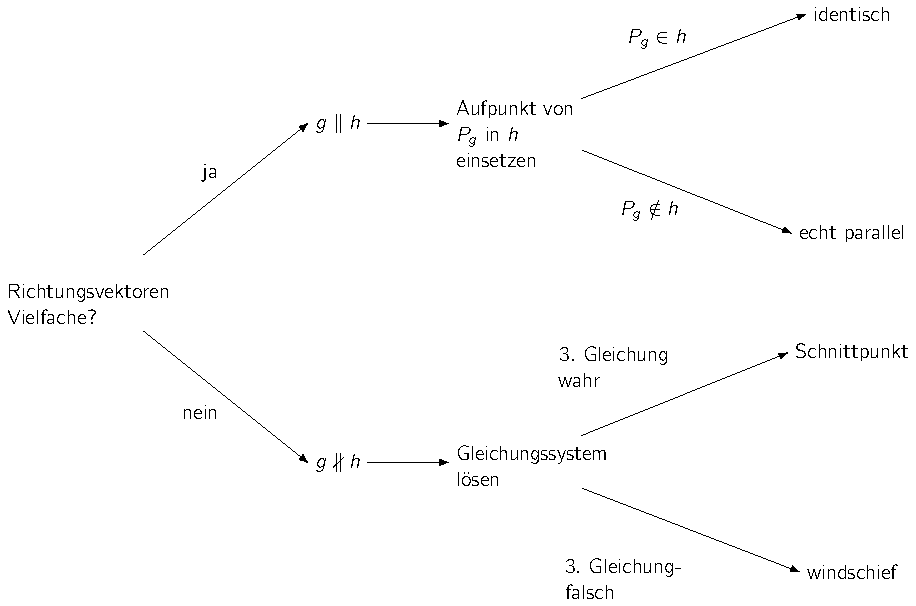
\includegraphics[width=11cm]{schema_gerade_gerade}
	
	
\end{antwort}	
\begin{frage}
	\LARGE
	Abstand zweier paralleler Geraden g und h
	
\end{frage}
\begin{antwort}
	\begin{itemize} 
		\item Funktioniert wie bei Abstand Punkt und Gerade
		\item Den Aufpunkt der Geraden h verwenden		
		\item Abstand vom Aufpunkt h zur Geraden g berechnen
	\end{itemize} 	
	
\end{antwort}	
\begin{frage}
	\LARGE
	Ebene durch die Punkte $A(1|2|-3)$, $B(6|2|2)$ und $C(8|-2|1)$
\end{frage}
\begin{antwort}
	
	$E:\vec{x}=\left(\begin{array}{c} 1 \\ 2 \\ -3\end{array} \right)+\lambda \cdot \left(\begin{array}{c} 5 \\ 0 \\ 5\end{array} \right)+\mu \cdot \left(\begin{array}{c} 7 \\-4 \\ 4\end{array} \right)$
	\bigskip
	
	$\hspace{2.2cm}\vec{A} \hspace{2.4cm} \vec{AB}  \hspace{2.2cm} \vec{AC}$
	
\end{antwort}		
\begin{frage}
	\LARGE
	Ebene durch den Punkt $P(2|2|-3)$ und $g:\vec{x}=\left(\begin{array}{c} 1 \\ 2 \\ 2\end{array} \right)+\lambda \cdot \left(\begin{array}{c} 4 \\ 2 \\ 5\end{array} \right)$
\end{frage}
\begin{antwort}
	
	$E:\vec{x}=\left(\begin{array}{c} 1 \\ 2 \\ 2\end{array} \right)+\lambda \cdot \left(\begin{array}{c} 4 \\ 2 \\ 5\end{array} \right)+\mu \cdot \left(\begin{array}{c} 1 \\0 \\ -5\end{array} \right)$
	\bigskip
	
	$\hspace{3cm} g  \hspace{4cm} \vec{A_gP}$
	
\end{antwort}	
\begin{frage}
	\LARGE
	Ebene durch zwei parallele Geraden
	\large
	$g:\vec{x}=\left(\begin{array}{c} 1 \\ 2 \\ 2\end{array} \right)+\lambda \cdot \left(\begin{array}{c} 4 \\ -2 \\ 2\end{array} \right)$
	
	$h:\vec{x}=\left(\begin{array}{c} 0 \\ -4 \\ 3\end{array} \right)+\mu \cdot \left(\begin{array}{c} 2 \\ -1 \\ 1\end{array} \right)$
\end{frage}
\begin{antwort}
	
	$E:\vec{x}=\left(\begin{array}{c} 1 \\ 2 \\ 2\end{array} \right)+\lambda \cdot \left(\begin{array}{c} 4 \\ -2 \\ 2\end{array} \right)+\mu \cdot \left(\begin{array}{c} -1 \\-6 \\ 1\end{array} \right)$
	\bigskip
	
	$\hspace{3cm} g  \hspace{4.5cm} \vec{A_gA_h}$
	
\end{antwort}	
\begin{frage}
	\LARGE
	Ebene durch zwei sich schneidende Geraden
	\large
	$g:\vec{x}=\left(\begin{array}{c} 1 \\ 2 \\ 2\end{array} \right)+\lambda \cdot \left(\begin{array}{c} 4 \\ -2 \\ 2\end{array} \right)$
	
	$h:\vec{x}=\left(\begin{array}{c} 5 \\ 0 \\ 4\end{array} \right)+\mu \cdot \left(\begin{array}{c} 3 \\ 0 \\ -1\end{array} \right)$
\end{frage}
\begin{antwort}
	
	$E:\vec{x}=\left(\begin{array}{c} 1 \\ 2 \\ 2\end{array} \right)+\lambda \cdot \left(\begin{array}{c} 4 \\ -2 \\ 2\end{array} \right)+\mu \cdot \left(\begin{array}{c} 3 \\0 \\ -1\end{array} \right)$
	\bigskip
	
	$\hspace{3cm} g  \hspace{4.5cm} \vec{v_h}$
	
\end{antwort}	
\begin{frage}
	\LARGE
	Gleichung einer Kugel
\end{frage}
\begin{antwort}
	
	$K: (x_1-m_1)^2+(x_2-m_2)^2+(x_3-m_3)^2=r^2$
	
	\begin{itemize} 
		\item $M(m_1|m_2|m_3)$ ist der Mittelpunkt der Kugel
		\item r ist der Radius der Kugel	
	\end{itemize} 
\end{antwort}	
\begin{frage}
	\LARGE
	Liegt ein Punkt P innerhalb, außerhalb oder auf der Kugel?
\end{frage}
\begin{antwort}
		
	\begin{enumerate} 
		\item Setze den Punkt in die Kugelgleichung ein
		\item Fasse zusammen
		\item\normalsize 	\begin{itemize}
				\item Linke Seite = Rechte Seite => P liegt auf der Kugel
				\item Linke Seite < Rechte Seite => P liegt innerhalb der Kugel
				\item Linke Seite > Rechte Seite => P liegt außerhalb der Kugel
				\end{itemize}	
	\end{enumerate} 
	
\end{antwort}	
\begin{frage}
	\LARGE
	Parameterform in Normalenform
	\bigskip
	
		$E:\vec{x}=\left(\begin{array}{c} 1 \\ 2 \\ 2\end{array} \right)+\lambda \cdot \left(\begin{array}{c} 4 \\ -2 \\ 2\end{array} \right)+\mu \cdot \left(\begin{array}{c} 3 \\0 \\ -1\end{array} \right)$
\end{frage}
\begin{antwort}
	\normalsize
	\begin{enumerate} 
		\item Kreuzprodukt der beiden Richtungsvektoren
		
		$\vec{n}=\left(\begin{array}{c} 4 \\ -2 \\ 2\end{array} \right) \times \left(\begin{array}{c} 3 \\0 \\ -1\end{array} \right)=\left(\begin{array}{c} 2 \\10 \\ 6\end{array} \right)$
		
		\item Normalenform hinschreiben: 
		
		$2 \cdot x_1 + 10 \cdot x_2+6 \cdot x_3 + c = 0$
		
		\item Aufpunkt A(1|2|2) einsetzen, um c zu erhalten: 
		
		$2 \cdot 1 + 10 \cdot 2+6 \cdot 2 + c = 0$
		... => c = -34
		
		\item Fertige Normalenform angeben: 
		
		$E: 2 \cdot x_1 + 10 \cdot x_2+6 \cdot x_3  -34 = 0$
			
	\end{enumerate} 
	
\end{antwort}
\begin{frage}
	\LARGE
	Normalenform in Parameterform
	
\end{frage}
\begin{antwort}
	\normalsize
	\begin{enumerate} 
		\item Schreibe für $x_1 = \lambda$ und für $x_2=\mu$	
		\item Setze in die Normalenform ein und löse nach $x_3$ auf.
		\item Sortiere jeweils in die entsprechenden Klammern der Ebene:			
	\end{enumerate} 
	$E:\vec{x}=\left(\begin{array}{c}  \\  \\ \end{array} \right)+\lambda \cdot \left(\begin{array}{c}  \\  \\ \end{array} \right)+\mu \cdot \left(\begin{array}{c}  \\ \\ \end{array} \right)$
	
\end{antwort}
\begin{frage}
	Ebenengleichungen der Koordinatenebenen
\end{frage}
\begin{antwort}

	\begin{itemize} 
		\item $x_1x_2-Ebene: x_3=0$	
		\item $x_1x_3-Ebene: x_2=0$
		\item $x_2x_3-Ebene: x_1=0$
	\end{itemize} 
	
\end{antwort}
\begin{frage}
	Welche besondere Lage haben die folgenden Ebenen im Raum?
	
	$E_1: 2 \cdot x_1+3  \cdot x_3  -12 = 0$
	
	$E_2: 4 \cdot x_3 +5 = 0$	
	
\end{frage}
\begin{antwort}
	
	\begin{itemize} 
		\item $E_1$: Parallel zur $x_2$-Achse	
		\item $E_2$: Parallel zur $x_1$- und $x_2$-Achse und damit parallel zur $x_1x_2$-Ebene
	\end{itemize} 
	\bigskip
	Merke: Immer parallel zu den x-Achsen, die fehlen.
	
\end{antwort}
\begin{frage}
	Schnittwinkel von Gerade g und Ebene E	
	
\end{frage}
\begin{antwort}
	
	\Large	
	\begin{itemize} 
		\item Der Schnittwinkel von Gerade und Ebene ergibt aus dem Winkel des Normalenvektors $\vec{n}$ der Ebene E und dem Richtungsvektor $\vec{v}$ von g.  
		\item => $sin(\alpha)=\frac{|\vec{n} \circ \vec{v}|}{|\vec{n}|\cdot|\vec{v}|}$
	\end{itemize} 	
\end{antwort}
\begin{frage}
	Lagebeziehungen von Gerade g und Ebene E	
	\Large
	
	(Die Ebene muss in Normalenform vorliegen! Wenn nötig umwandeln.)
\end{frage}
\begin{antwort}
	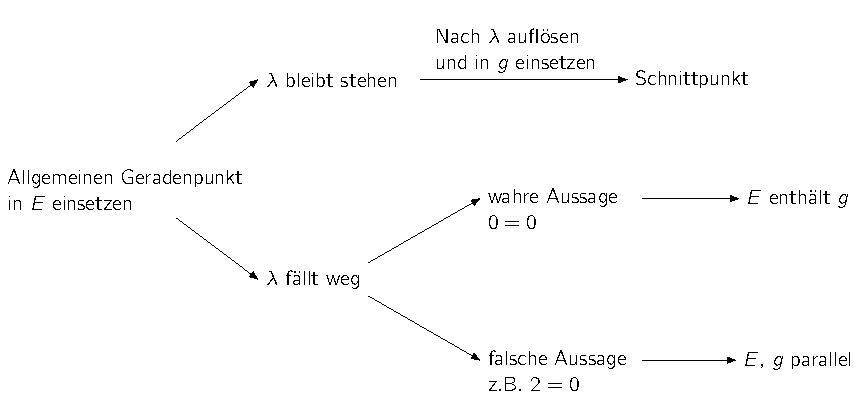
\includegraphics[width=13cm]{schema_ebene_gerade}
\end{antwort}
\begin{frage}
	Abstand Punkt - Ebene
	
	Bsp: P(1|1|2),
	
	E: $2x_1 + 2x_2+ x_3 + 6=0$
\end{frage}
\begin{antwort}
	\LARGE
	$d=\frac{|n_1 \cdot x_1 + n_2 \cdot x_2+ n_3 \cdot x_3 + c|}{|\vec{n}|}$
	
	\bigskip
	\large
	$d=\frac{|2 \cdot x_1 + 2 \cdot x_2+ x_3 + 6|}{|\vec{n}|}$
	$=\frac{|2 \cdot x_1 + 2 \cdot x_2+ x_3 + 6|}{\sqrt{2^2+2^2+1^2}}$
	$=\frac{|2 \cdot x_1 + 2 \cdot x_2+ x_3 + 6|}{3}$
	
	\bigskip
	P einsetzen:
	$d=\frac{|2 \cdot 1 + 2 \cdot 1+ 2 + 6|}{3}=4$
	
\end{antwort}
\begin{frage}
	Abstand von einer parallelen Geraden g zur Ebene E
	
\end{frage}
\begin{antwort}
	\begin{itemize} 
		\item Der Abstand ist überall gleich
		\item Es genügt den Abstand vom Aufpunkt der Geraden g zur Ebene E zu bestimmen
		\item Selbes Vorgehen wie bei 'Abstand Punkt-Ebene'	
	\end{itemize} 
	
\end{antwort}
\begin{frage}
	Schnittpunkt einer Geraden g mit einer Ebene E
	
\end{frage}
\begin{antwort}
	\begin{itemize} 
		\item Allgemeinen Geradenpunkt G bestimmen
		\item Geradenpunkt G in die Ebene für $x_1$, $x_2$ und $x_3$ einsetzten und $\lambda$ ausrechnen
		\item $\lambda$ in Geradenpunkt G einsetzen
		
		 => Schnittpunkt S
	\end{itemize}
	
\end{antwort}
\begin{frage}
	Lotfußpunkt von P auf eine Ebene E
	
\end{frage}
\begin{antwort}
	\Large	
	\begin{enumerate} 
		\item Stelle zunächst eine Hilfsgerade auf:
		\begin{itemize} 
			\item Verwende P als Aufpunkt
			\item Verwende den Normalenvektor von E als Richtungsvektor
		\end{itemize} 		  
		\item Berechne den Schnittpunkt der Hilfsgeraden mit der Ebene
		\item Der Schnittpunkt ist zugleich der Lotfußpunkt F
	\end{enumerate} 	
\end{antwort}
\begin{frage}
	Abstand zweier paralleler Ebenen E und F
	
\end{frage}
\begin{antwort} 
	\begin{enumerate} 
		\item Der Abstand ist überall gleich
		\item Es genügt den Abstand vom Aufpunkt der Ebene F zur Ebene E zu bestimmen
		\item Selbes Vorgehen wie bei 'Abstand Punkt-Ebene'	
	\end{enumerate} 
	
\end{antwort}
\begin{frage}
	Schnittwinkel zweier Ebenen E und F	
	
\end{frage}
\begin{antwort}
	
	\Large	
	\begin{itemize} 
		\item Der Schnittwinkel zweier Ebenen ergibt sich aus dem Schnittwinkel der beiden Normalenvektoren $\vec{n_E}$ der Ebene E und $\vec{n_F}$ der Ebene F.  
		\item => $cos(\alpha)=\frac{|\vec{n_E} \circ \vec{n_F}|}{|\vec{n_E}|\cdot|\vec{n_F}|}$
	\end{itemize} 	
\end{antwort}
\begin{frage}
	Schnittgerade zweier Ebenen E (in Normalenform) und F (in Parameterform)	
	
\end{frage}
\begin{antwort}
	\Large	
	\begin{enumerate} 
		\item Eine der Ebenen muss in Normalenform, die andere in Parameterform gegeben sein.
		\item Allgemeinen Ebenenpunkt von F bestimmen und in E einsetzen
		\item Nach $\lambda$ (oder $\mu$) auflösen und in die Parameterform einsetzen
		\item Vereinfachen und zusammenfassen => Schnittgerade s
	\end{enumerate} 	
\end{antwort}
\begin{frage}
	Lage zweier Ebenen E und F
	
\end{frage}
\begin{antwort} 
	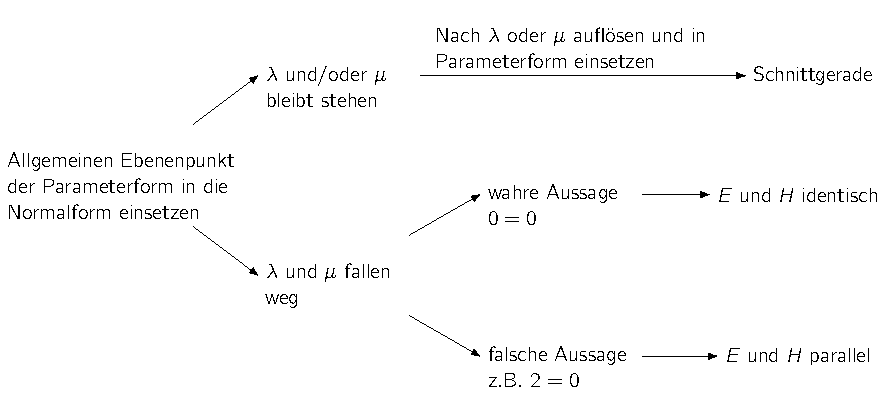
\includegraphics[width=13cm]{schema_ebene_ebene} 
	
\end{antwort}
\begin{frage}
	Punkt an einer Gerade oder Ebene spiegeln	
	
\end{frage}
\begin{antwort}
	\Large	
	\begin{enumerate} 
		\item Lotfußpunkt F berechnen
		\item F in folgende 'Spiegelformel' einsetzen:
		
		$\vec{P^*}=\vec{P}+2 \cdot \vec{PF}$
	\end{enumerate} 	
\end{antwort}
\end{document}